% CVPR 2024 Paper Template; see https://github.com/cvpr-org/author-kit

\documentclass[10pt,twocolumn,letterpaper]{article}

%%%%%%%%% PAPER TYPE  - PLEASE UPDATE FOR FINAL VERSION
\usepackage{cvpr}              % To produce the CAMERA-READY version
% \usepackage[review]{cvpr}      % To produce the REVIEW version
% \usepackage[pagenumbers]{cvpr} % To force page numbers, e.g. for an arXiv version

% Import additional packages in the preamble file, before hyperref
%
% --- inline annotations
%
\usepackage[dvipsnames]{xcolor}
\newcommand{\red}[1]{{\color{red}#1}}
\newcommand{\todo}[1]{{\color{red}#1}}
\newcommand{\TODO}[1]{\textbf{\color{red}[TODO: #1]}}
% --- disable by uncommenting  
% \renewcommand{\TODO}[1]{}
% \renewcommand{\todo}[1]{#1}



% It is strongly recommended to use hyperref, especially for the review version.
% hyperref with option pagebackref eases the reviewers' job.
% Please disable hyperref *only* if you encounter grave issues, 
% e.g. with the file validation for the camera-ready version.
%
% If you comment hyperref and then uncomment it, you should delete *.aux before re-running LaTeX.
% (Or just hit 'q' on the first LaTeX run, let it finish, and you should be clear).
\definecolor{cvprblue}{rgb}{0.21,0.49,0.74}
\usepackage[pagebackref,breaklinks,colorlinks,citecolor=cvprblue]{hyperref}

%%%%%%%%% PAPER ID  - PLEASE UPDATE
\def\paperID{*****} % *** Enter the Paper ID here
\def\confName{CVPR}
\def\confYear{2024}

%%%%%%%%% TITLE - PLEASE UPDATE
\title{DynTCG: Dynamic View Synthesis from Monocular RGBD Streams via Flow-Tracked Compact Gaussians}

%%%%%%%%% AUTHORS - PLEASE UPDATE
\author{Zhehao Shen\\
2021533110\\
{\tt\small shenzhh@shanghaitech.edu.cn}
% For a paper whose authors are all at the same institution,
% omit the following lines up until the closing ``}''.
% Additional authors and addresses can be added with ``\and'',
% just like the second author.
% To save space, use either the email address or home page, not both
\and
Penghao Wang\\
2021533138\\
{\tt\small wangph1@shanghaitech.edu.cn}
\and
Yu Hong\\
2021533148\\
{\tt\small hongyu@shanghaitech.edu.cn}
\and
Zhirui Zhang\\
2021533024\\
{\tt\small zhangzhr4@shanghaitech.edu.cn}
\and
Shouchen Zhou\\
2021533042\\
{\tt\small zhoushch@shanghaitech.edu.cn}
}

\usepackage{graphicx}
\usepackage{amsmath}
\usepackage{multirow}
\usepackage{booktabs}
\usepackage{lipsum}
\usepackage{colortbl}

\newcommand{\highlightBest}[1]{\colorbox[rgb]{.866,.945, 0.831}{#1}}
\newcommand{\bestCellColor}[1]{\cellcolor[rgb]{.866,.945, 0.831}#1}

\newcommand{\highlightSecondBest}[1]{\colorbox[rgb]{1, 0.98, 0.83}{#1}}
\newcommand{\secondBestCellColor}[1]{\cellcolor[rgb]{1, 0.98, 0.83}#1}
% 255 224 218
\newcommand{\highlightThirdBest}[1]{\colorbox[rgb]{1, 0.87, 0.85}{#1}}
\newcommand{\thirdBestCellColor}[1]{\cellcolor[rgb]{1, 0.87, 0.85}{#1}}


\begin{document}
\maketitle
% \begin{abstract}

In this assignment, we implemented the NeRF and its accelerate method to do 3D novel view synthesis. And we tested the methods on our own datasets, and try to merge the different accelerate methods to chase for a better performance. 

And the following tasks were finished.
\begin{itemize}
    \item Task1: Implementation of NeRF accelerate method (TensoRF and NGP)
    \item Task2: Processing of our own $3$ custom dataset and dataloader of it, then test the performance.
    \item Task3: improve the performance by reasonably combining NGP and TensoRF.
\end{itemize}

\end{abstract}    
% \section{Introduction}



% \section{Formatting your paper}
\label{sec:formatting}

All text must be in a two-column format.
The total allowable size of the text area is $6\frac78$ inches (17.46 cm) wide by $8\frac78$ inches (22.54 cm) high.
Columns are to be $3\frac14$ inches (8.25 cm) wide, with a $\frac{5}{16}$ inch (0.8 cm) space between them.
The main title (on the first page) should begin 1 inch (2.54 cm) from the top edge of the page.
The second and following pages should begin 1 inch (2.54 cm) from the top edge.
On all pages, the bottom margin should be $1\frac{1}{8}$ inches (2.86 cm) from the bottom edge of the page for $8.5 \times 11$-inch paper;
for A4 paper, approximately $1\frac{5}{8}$ inches (4.13 cm) from the bottom edge of the
page.

%-------------------------------------------------------------------------
\subsection{Margins and page numbering}

All printed material, including text, illustrations, and charts, must be kept
within a print area $6\frac{7}{8}$ inches (17.46 cm) wide by $8\frac{7}{8}$ inches (22.54 cm)
high.
%
Page numbers should be in the footer, centered and $\frac{3}{4}$ inches from the bottom of the page.
The review version should have page numbers, yet the final version submitted as camera ready should not show any page numbers.
The \LaTeX\ template takes care of this when used properly.



%-------------------------------------------------------------------------
\subsection{Type style and fonts}

Wherever Times is specified, Times Roman may also be used.
If neither is available on your word processor, please use the font closest in
appearance to Times to which you have access.

MAIN TITLE.
Center the title $1\frac{3}{8}$ inches (3.49 cm) from the top edge of the first page.
The title should be in Times 14-point, boldface type.
Capitalize the first letter of nouns, pronouns, verbs, adjectives, and adverbs;
do not capitalize articles, coordinate conjunctions, or prepositions (unless the title begins with such a word).
Leave two blank lines after the title.

AUTHOR NAME(s) and AFFILIATION(s) are to be centered beneath the title
and printed in Times 12-point, non-boldface type.
This information is to be followed by two blank lines.

The ABSTRACT and MAIN TEXT are to be in a two-column format.

MAIN TEXT.
Type main text in 10-point Times, single-spaced.
Do NOT use double-spacing.
All paragraphs should be indented 1 pica (approx.~$\frac{1}{6}$ inch or 0.422 cm).
Make sure your text is fully justified---that is, flush left and flush right.
Please do not place any additional blank lines between paragraphs.

Figure and table captions should be 9-point Roman type as in \cref{fig:onecol,fig:short}.
Short captions should be centred.

\noindent Callouts should be 9-point Helvetica, non-boldface type.
Initially capitalize only the first word of section titles and first-, second-, and third-order headings.

FIRST-ORDER HEADINGS.
(For example, {\large \bf 1. Introduction}) should be Times 12-point boldface, initially capitalized, flush left, with one blank line before, and one blank line after.

SECOND-ORDER HEADINGS.
(For example, { \bf 1.1. Database elements}) should be Times 11-point boldface, initially capitalized, flush left, with one blank line before, and one after.
If you require a third-order heading (we discourage it), use 10-point Times, boldface, initially capitalized, flush left, preceded by one blank line, followed by a period and your text on the same line.

%-------------------------------------------------------------------------
\subsection{Footnotes}

Please use footnotes\footnote{This is what a footnote looks like.
It often distracts the reader from the main flow of the argument.} sparingly.
Indeed, try to avoid footnotes altogether and include necessary peripheral observations in the text (within parentheses, if you prefer, as in this sentence).
If you wish to use a footnote, place it at the bottom of the column on the page on which it is referenced.
Use Times 8-point type, single-spaced.


%-------------------------------------------------------------------------
\subsection{Cross-references}

For the benefit of author(s) and readers, please use the
{\small\begin{verbatim}
  \cref{...}
\end{verbatim}}  command for cross-referencing to figures, tables, equations, or sections.
This will automatically insert the appropriate label alongside the cross-reference as in this example:
\begin{quotation}
  To see how our method outperforms previous work, please see \cref{fig:onecol} and \cref{tab:example}.
  It is also possible to refer to multiple targets as once, \eg~to \cref{fig:onecol,fig:short-a}.
  You may also return to \cref{sec:formatting} or look at \cref{eq:also-important}.
\end{quotation}
If you do not wish to abbreviate the label, for example at the beginning of the sentence, you can use the
{\small\begin{verbatim}
  \Cref{...}
\end{verbatim}}
command. Here is an example:
\begin{quotation}
  \Cref{fig:onecol} is also quite important.
\end{quotation}

%-------------------------------------------------------------------------
\subsection{References}

List and number all bibliographical references in 9-point Times, single-spaced, at the end of your paper.
When referenced in the text, enclose the citation number in square brackets, for
example~\cite{Authors14}.
Where appropriate, include page numbers and the name(s) of editors of referenced books.
When you cite multiple papers at once, please make sure that you cite them in numerical order like this \cite{Alpher02,Alpher03,Alpher05,Authors14b,Authors14}.
If you use the template as advised, this will be taken care of automatically.

\begin{table}
  \centering
  \begin{tabular}{@{}lc@{}}
    \toprule
    Method & Frobnability \\
    \midrule
    Theirs & Frumpy \\
    Yours & Frobbly \\
    Ours & Makes one's heart Frob\\
    \bottomrule
  \end{tabular}
  \caption{Results.   Ours is better.}
  \label{tab:example}
\end{table}

%-------------------------------------------------------------------------
\subsection{Illustrations, graphs, and photographs}
\begin{table}[b]
    \Huge
	\begin{center}
		\centering
		\caption{Quantitative evaluation of NeRF accelerating methods.}
		\label{table:quantitative}
		\resizebox{0.45\textwidth}{!}{
			\begin{tabular}{l|c|c}
				\hline
				\hline
& Per-frame Storage(MB) $\downarrow$ & PSNR(dB) $\uparrow$\\
\hline
Raw Point Cloud   &  46.23 & 32.47  \\
% \hline
High-bit Quantization    &  7.34 & 32.23  \\
% \hline
Low-bit Quantization    &  3.23 & 29.56  \\
% \hline
\hline
Ours Residual Encoding    &  1.35 & 32.30  \\
\hline
\hline
			\end{tabular}
		}
		\vspace{-20pt}
	\end{center}
\end{table}
\begin{table}[b]
    \Huge
	\begin{center}
		\centering
		\caption{Quantitative evaluation of NeRF accelerating methods.}
		\label{table:quantitative}
		\resizebox{0.45\textwidth}{!}{
			\begin{tabular}{l|c|c}
				\hline
				\hline
&Training (min) $\downarrow$ & PSNR(dB) $\uparrow$\\
\hline
Without Flow Tracking  &  93.23 & 31.65  \\
% \hline
Ours-full(before compression)     &  70.34 & 32.47  \\
% \hline
\hline
Ours-full(after compression)     &  70.64 & 32.30 \\
% \hline
\hline
\hline
			\end{tabular}
		}
		\vspace{-20pt}
	\end{center}
\end{table}
All graphics should be centered.
In \LaTeX, avoid using the \texttt{center} environment for this purpose, as this adds potentially unwanted whitespace.
Instead use
{\small\begin{verbatim}
  \centering
\end{verbatim}}
at the beginning of your figure.
Please ensure that any point you wish to make is resolvable in a printed copy of the paper.
Resize fonts in figures to match the font in the body text, and choose line widths that render effectively in print.
Readers (and reviewers), even of an electronic copy, may choose to print your paper in order to read it.
You cannot insist that they do otherwise, and therefore must not assume that they can zoom in to see tiny details on a graphic.

When placing figures in \LaTeX, it's almost always best to use \verb+\includegraphics+, and to specify the figure width as a multiple of the line width as in the example below
{\small\begin{verbatim}
   \usepackage{graphicx} ...
   \includegraphics[width=0.8\linewidth]
                   {myfile.pdf}
\end{verbatim}
}


%-------------------------------------------------------------------------
\subsection{Color}

Please refer to the author guidelines on the \confName\ \confYear\ web page for a discussion of the use of color in your document.

If you use color in your plots, please keep in mind that a significant subset of reviewers and readers may have a color vision deficiency; red-green blindness is the most frequent kind.
Hence avoid relying only on color as the discriminative feature in plots (such as red \vs green lines), but add a second discriminative feature to ease disambiguation.
\begin{abstract}

We present a method that uses deformable Gaussian representation based on monocular RGBD input, aimed at accomplishing the task of 
dynamic novel view synthesis. The 2D images with depth are back-projected into 3D point clouds to initialize Gaussians, and the flow between frames is utilized to generate warped Gaussians as the priors of the deformable network. RANS encoding and quantization were also used to do residue compress for improvements. Our method balanced the training, rendering time, and quantities of novel view, achieving monocular dynamic novel view synthesis.
\end{abstract}

\begin{figure*}[t] 
	\begin{center} 
		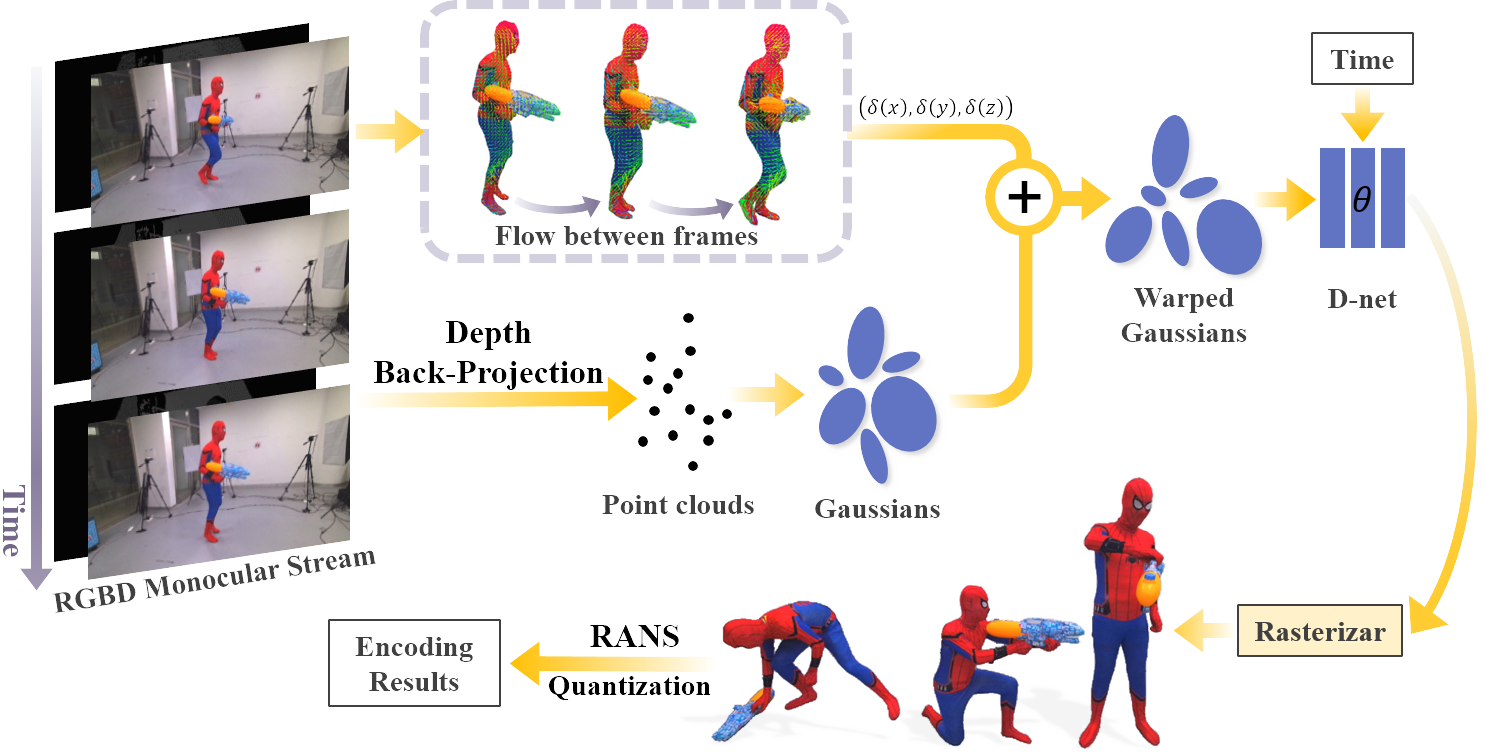
\includegraphics[width=\linewidth]{sec/fig/pipeline.png} 
	\end{center} 
    \vspace{-20pt}  
% (a)我们的setting是RGBD monocular stream (b)对depth反投影产生初始点云初始化gaussians (c)利用flow between frames对gaussians进行warp,得到的warped gaussians作为先验进入deformable net(D-net)(d)D-net额外引入time作为输入估计当前的deltax,deltay,deltaz,deltar (e)对得到的gaussians利用RANS和quantization进行压缩
    \caption{\noindent{\bf Overview of DynTCG.} (a) Our setting involves an RGBD monocular stream. (b) DynTCG performs back-projection on the depth to generate initial point clouds and initialize Gaussians. (c) Utilizing the flow between frames, we warp the Gaussians, and the resulting warped Gaussians are used as a prior input into the deformable network (D-net). (d) The D-net additionally introduces time as an input to estimate the current $\delta(x)$, $\delta(y)$, $\delta(z)$, and $\delta(r)$. (e) After training, the Gaussians are then compressed using RANSAC and quantization.}
	\label{fig:fig_2_overview} 
	\vspace{-8pt}
\end{figure*} 


\section{Introduction}
The precise reconstruction and photorealistic rendering of dynamic scenes from a collection of input images are paramount for numerous applications, such as augmented reality/virtual reality (AR/VR) and 3D content production. In these contexts, achieving high-quality results is essential for an immersive and visually convincing experience. 

% The original radiance methods such as NeRF methods usually have the slower training and rendering speed with with equivalent quality, so the Gaussian-splatting technique was introduced to improve training efficiency, achieved the balance between speed and quantity.
However, the multi-view setting remains impractical for everyday consumer use. In contrast, the monocular method, utilizing a single and convenient commercial RGBD camera, proves to be more practical and appealing for daily applications.

Recent advancements in neural rendering, exemplified by Neural Radiance Fields (NeRF)\cite{mildenhall2020nerf}, have facilitated photorealistic rendering with dense-view supervision. Particularly noteworthy are dynamic variants of NeRF~\cite{gao2021dynamic}, which excel in synthesizing compelling novel views of dynamic scenes, even when captured monocularly. However, these approaches depend on laborious and time-consuming per-scene training to seamlessly integrate temporal observations into the canonical space.

The recent development known as 3D Gaussian Splatting (3DGS) 
~\cite{kerbl3Dgaussians} reverts to an explicit paradigm for representing static scenes. Utilizing GPU-friendly rasterization of 3D Gaussian primitives, it enables real-time and high-quality rendering of radiance fields that were unprecedented until now.

In this paper, we propose DynTCG, a novel approach for synthesizing novel views of dynamic scenes based on flow-tracked and compact Gaussian representations, utilizing monocular dynamic RGBD input. Our key idea involves leveraging the powerful prior provided by flow tracking of 2D images and depth information as the deform field for dynamic Gaussians. Simultaneously, we discovered that optimizing the scaling of Gaussians in the deform-net has minimal impact on appearance and can even affect training speed. Consequently, we modified the deform-net, originally designed in the baseline to optimize position, rotation, and scaling simultaneously. The adjustment now focuses solely on optimizing position and rotation. This alteration aims to enhance training speed with almost negligible impact on rendering quality. Given the substantial storage overhead associated with Gaussians (requiring storage of 3rd-order spherical harmonics coefficients for each point and information for modeling Gaussian scale, position, rotation, and opacity), we introduce a quantization and entropy encoding-based residual compression method tailored for dynamic scenes. This approach transforms the representation of Gaussians into a more compact form, thereby significantly reducing storage requirements.





To summarize, our main contributions include:
 
\begin{itemize}
    \item We propose a deformable Gaussian representation based on 
monocular RGBD input, aimed at accomplishing the task of 
dynamic novel view synthesis.
    \item We observed that optimizing scaling in the deform-net doesn't significantly impact the final rendering of dynamic scenes. On the contrary, it tends to affect training speed. Therefore, we have removed the optimization of scaling from the deform-net。
    \item Utilizing optical flow tracking from 2D images, we provide an 
optimized initialization for the dynamic Gaussian deform field, 
significantly accelerating the training speed and enhancing 
the rendering quality under a monocular setting.
    \item We showcase a companion compression scheme, 
supporting high-quality rendering with low storage, even 
under various platforms.
\end{itemize}

Our method achieves less training time, better rendering quantity, and less per-frame storage, which greatly balances the time consumption and the rendering quality.




\section{Method}\label{sec:algorithm} 
Utilizing RGBD monocular streams captured by a Kinect camera, DynTCG seamlessly integrates recent advancements in differentiable rasterization with tracking flow and deformable fields\cite{yang2023deformable3dgs}. This innovative blend not only enhances the optimization process but also significantly improves the rendering quality. Moreover, our approach demonstrates remarkable performance in terms of storage efficiency. A visual summary of our methodology can be found in Fig.~\ref{fig:fig_2_overview}.

Our approach begins with the creation of an initial point cloud via depth back-projection, followed by the initialization of Gaussians. Concurrently, we project these Gaussians onto pixels and establish the warped relationship between Gaussian point clouds across frames using a pixel tracking method between consecutive frames. This results in the creation of warped Gaussians, which serve as a prior for the deformable network. The deformable network utilizes these warped Gaussians and time as inputs to estimate the changes in position and rotation of the Gaussians, thereby training temporal Gaussians. Furthermore, we introduce a novel compression scheme. This scheme significantly reduces storage needs, enabling the immersive viewing of high-fidelity human performances with a storage requirement of less than 2 MB per frame.

\subsection{Flow tracking}
Inspired by Instant-NVR~\cite{jiang2023instantnvr}, we aim to enhance the training speed and rendering effectiveness of the deform field by introducing a geometric constraint as a robust prior. While the ed node employed in Instant-NVR represents a powerful geometric prior, its integration into the Gaussian code proves to be challenging. Drawing further inspiration from the approach in dynamic nerf~\cite{gao2021dynamic}, which utilizes optical flow to provide prior information, we integrate optical flow into the Gaussian training pipeline. This involves calculating the $\delta x$ and $\delta y$ from optical flow derived from the 2D image, along with $\delta z$ information from the depth image. Through projection and back-projection calculations, we obtain a prior for the deform net.
\begin{figure}[t] 
	\begin{center} 
		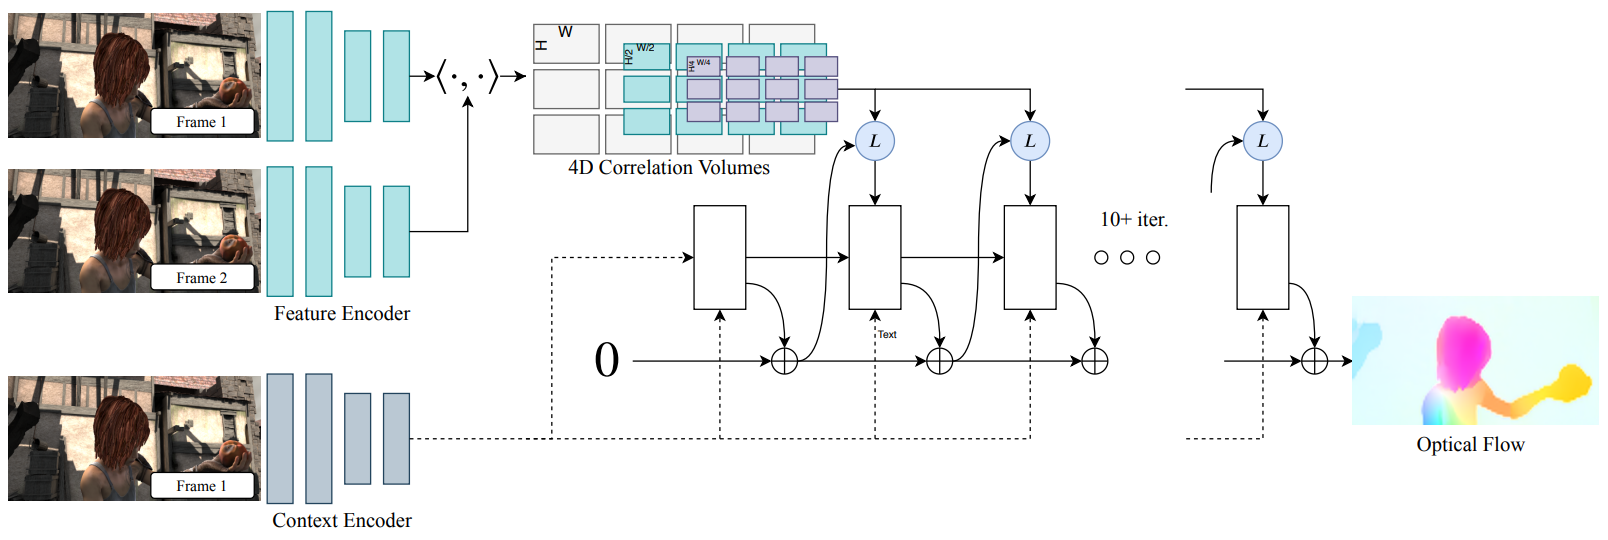
\includegraphics[width=\linewidth]{sec/fig/RAFT.png} 
	\end{center} 
    \vspace{-20pt}
    \caption{\noindent{\bf Pipeline of RAFT}: containing Feature Extractor \& Context Extractor, Visual Similarity Calculator and Updater}
    \label{fig:hello}
\end{figure}
We employ RAFT~\cite{10.1007/978-3-030-58536-5_24} as our method for optical flow tracking. RAFT comprises a Feature Extractor, Context Extractor, Visual Similarity Calculator, and Updater to optimize the flow tracking process. The pipeline of RAFT is shown in Fig.~\ref{fig:hello}.
\\
\textbf{Feature Extractor \& Context Extractor } extract features from two images, followed by the extraction of semantic information from one of the images.
\\
\textbf{Visual Similarity Calculator }constructs a 4D correlation volume by calculating the dot product between feature vectors.
\\
\textbf{Updater }updates and refines flow tracking by iteratively searching the correlation volume based on current optical flow estimates.

\begin{figure}[b]
	\centering
	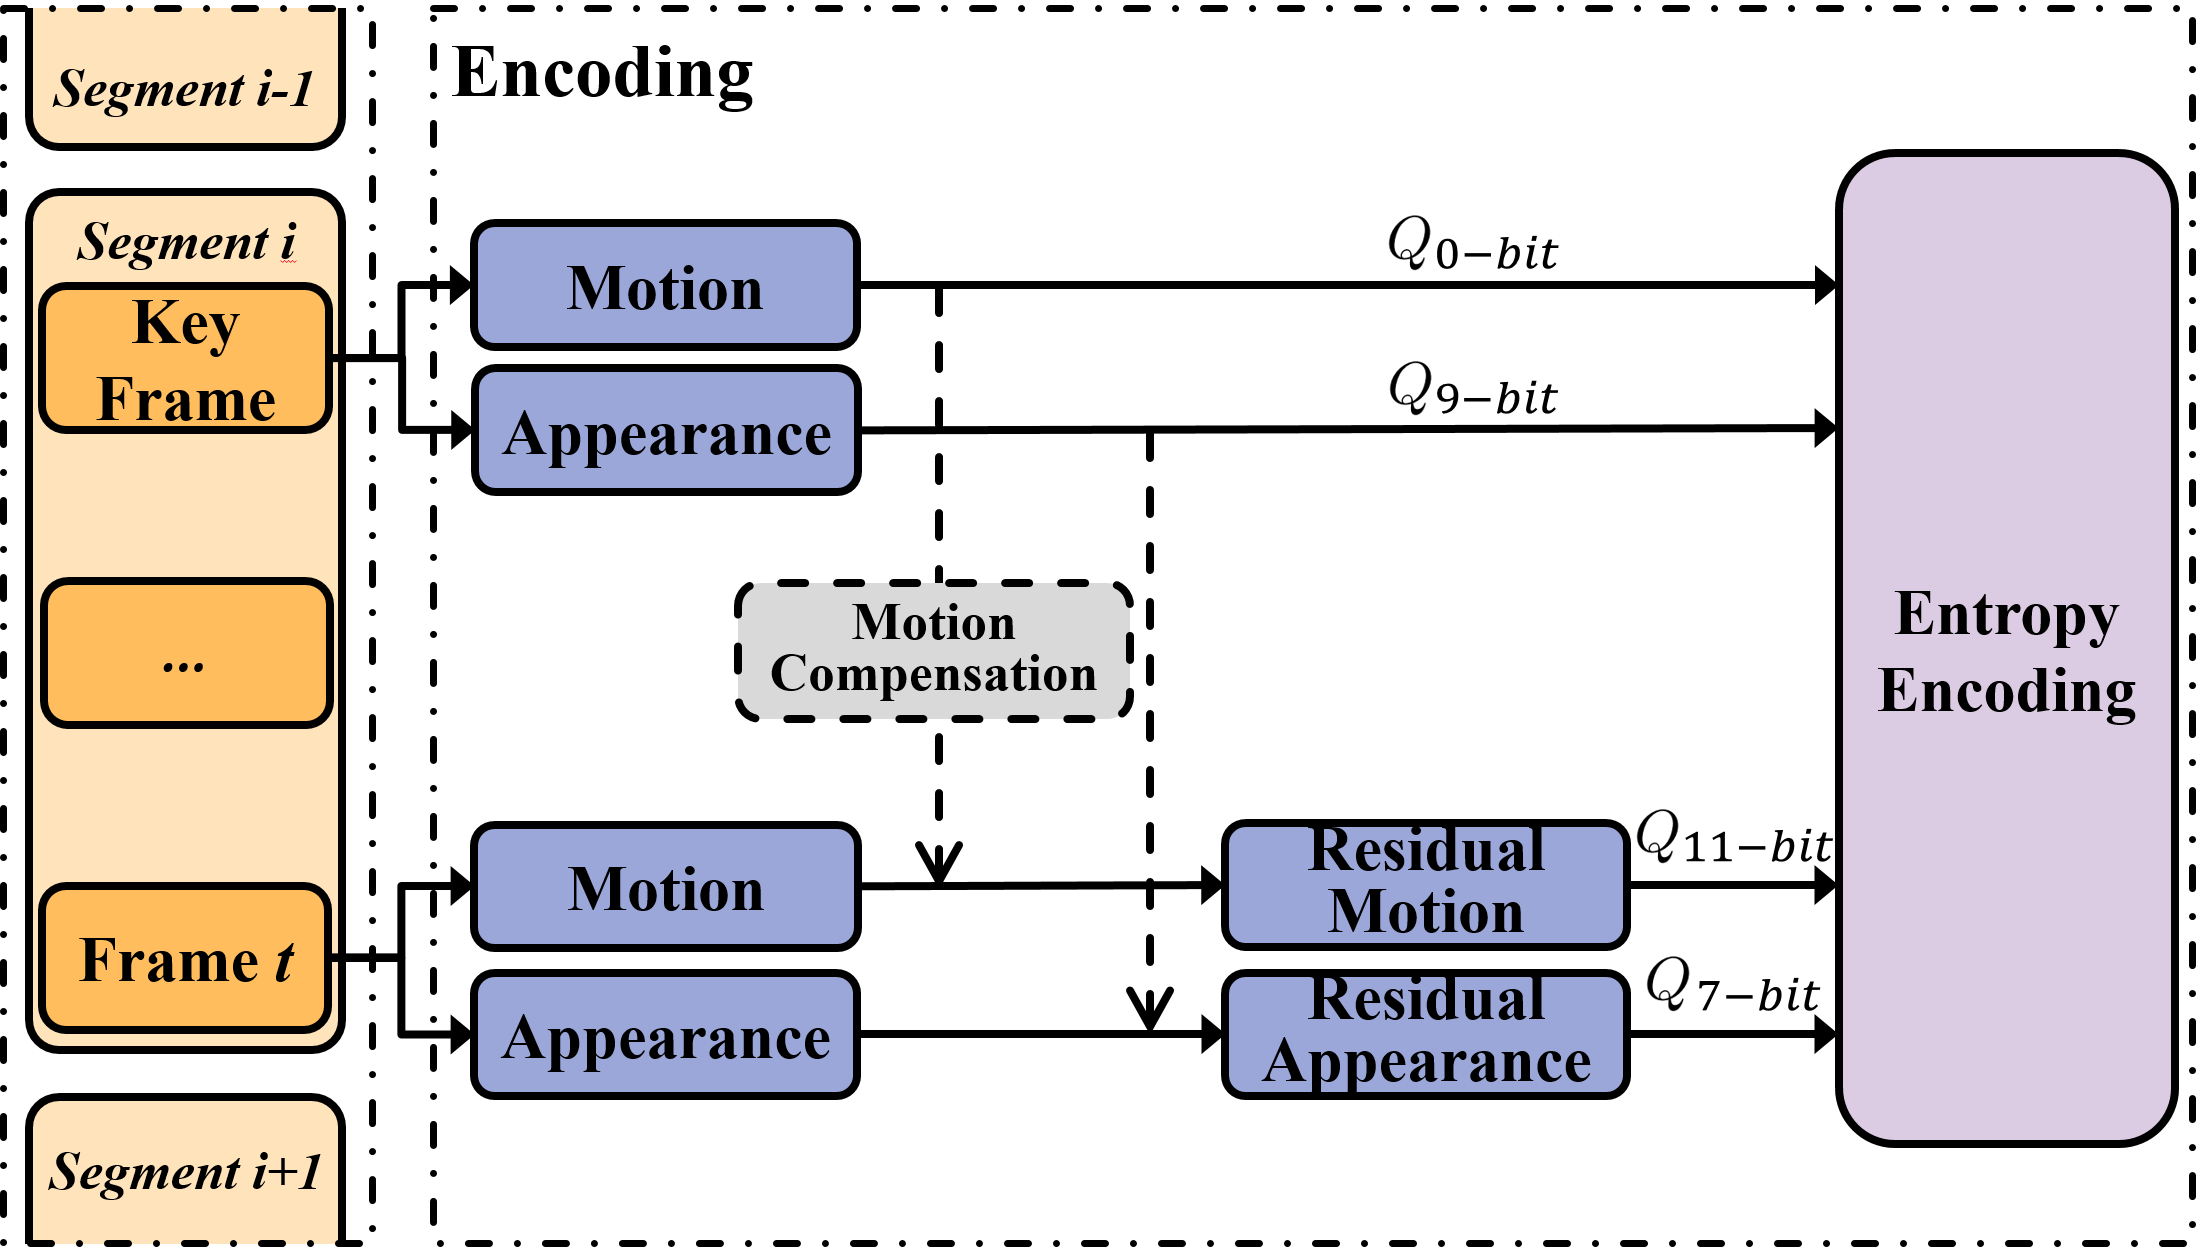
\includegraphics[width=\linewidth]{sec/fig/encoding.png}
	\vspace{-20pt}
	\caption{Illustration of residual encoding strategy for DynTCG.}
	\label{fig:encoding}
\end{figure}
\subsection{Compact 4D Gaussians}
After Gaussian optimization, we dump the Gaussian splat points and the deformation network into separate frame Gaussian splat points. However, storage of 64-dimensional with a 3-order sh coefficient takes large disk storage, making it hard to store long dynamic sequences. To address this, we present a Residual Compression method as shown in Fig.~\ref{fig:encoding}, including residual computation, quantization, and RANS encoding. 

\noindent{\bf Residual Compression}
For dynamic sequences, adjacent frames share similar Gaussian point parameters in a set of frames. We split the whole sequence into several segments and the object's movement is relatively small, then we compute the residual data between each frame and the first frame, such that the residual data distribution range of data will be much smaller. Then we apply compression separately to motion and appearance. 

\noindent{\bf Quantization}
As for the residual data, we perform quantization separately to the delta position and delta appearance. As motion needs higher precision to maintain rendering quality, we adopt a lower quantization bit on the position attribute. We need to ensure the precision for the first frame, so we do not perform quantization to the first frame position and perform 9-bit quantization to appearance to ensure the base frame precision. For other frames in this segment, we adopt 11-bit quantization to delta position and 7-bit quantization to delta appearance. 

\noindent{\bf RANS Encoding}
After quantization of the float number to an integer number, we perform RANS encoding to compress the data. This entropy encoding system encodes each attribute by calculating the numerical distribution frequency and finally encodes the attribute to an integer stream. 
By using our residual encoding method, we could compress the Gaussian point cloud efficiently by 20 times on the storage, which addresses long dynamic sequences on low disk storage and fast data transport. 

\section{Implementation Details}\label{sec:detail} 

Firstly, for data obtained from HyperNeRF\cite{park2021hypernerf} and DynamicNeRF\cite{gao2021dynamic} datasets, we leverage the state-of-the-art single-image depth estimation\cite{Ranftl2022} to estimate the input depth. Our approach to the deformable field is inspired by the work of Ziyi Yang\cite{yang2023deformable3dgs} and is based on a broad framework of 3D Gaussians\cite{kerbl3Dgaussians}.

Regarding the training process, we conducted a total of 40,000 iterations. In the initial 3,000 iterations, we solely trained the 3D Gaussians to attain relatively stable positions and shapes. Following this phase, we commenced the joint training of both the 3D Gaussians and the deformation field. A single Adam optimizer\cite{kingma2017adam}, was utilized for optimization purposes.
During compression, we first quantize the appearance attributes, then fix these parameters and fine-tune motion $p$ and $q$ of 4D Gaussians over an additional 1000 iterations. Afterward, we quantize the motion. To mitigate the influence of quantization on the outcomes, We apply different precision levels for various attributes to balance storage and quality.

All the experiments were done on 4 Nvidia 2080Ti.


% We implement our framework using PyTorch [32] and modify the differentiable Gaussian rasterization by incorporating depth visualization. For training, we conducted training for a total of 40k iterations. During the initial 3k iterations, we solely trained the 3D Gaussians to attain relatively
% stable positions and shapes. Subsequently, we jointly train
% the 3D Gaussians and the deformation field. For optimization, a single Adam optimizer [17] is used but with a different learning rate for each component: the learning rate of
% 3D Gaussians is exactly the same as the official implementation, while the learning rate of the deformation network
% undergoes exponential decay, ranging from 8e-4 to 1.6e-6.
% Adam’s β value range is set to (0.9, 0.999). Experiments
% with synthetic datasets were all conducted against a black
% background and at a full resolution of 800x800. All the experiments were done on an NVIDIA RTX 3090.

\begin{figure*}[t] 
	\begin{center} 
        \vspace{10pt}
		\includegraphics[width=\linewidth]{sec/fig/comparison.png} 
	\end{center} 
    \vspace{-15pt}
    \caption{Qualitative comparison against monocular dynamic scene reconstruction methods}
	\label{fig:comparison} 
\end{figure*} 

\section{Experiments}
\subsection{Ablation}
\noindent{\bf Flow Tracking Prior}
We conduct a qualitative ablation on the flow tracking prior to assess its impact on rendering results. As shown in Tab.~\ref{table:quantitative}, omitting the flow tracking prior and relying solely on the deform net tends to prolong the training time. In contrast, our full pipeline enhances the preprocessing of images to establish flow between frames. This approach integrates depth and optical flow, serving as an efficient initialization method for the deform net, aiming to expedite the optimization process.

% We conduct a qualitative ablation
% on the dual-graph and the regularization term to assess their
% impact on post-compression rendering results. As shown in
% Fig. 6, the removal of the coarse ED-graph prior typically
% causes severe artifacts. Excluding the Gaussian graph of-
% ten results in significant precision loss and unnatural render-
% ing. Regarding regularizers, the omission of Etemp usually
% triggers unrealistic artifacts post-compression. Meanwhile,
% the absence of Esmooth produces blurry results, with both
% leading to flickering in the video. Additionally, to evalu-
% ate the impact of the adaptive weight wi,t, we replace it
% with a fixed weight of 0.1. This adjustment generally leads
% to noticeable blurriness, especially in areas with significant
% movement. In contrast, our full pipeline generates spatially
% and temporally compact 4D Gaussians, maintaining high-
% fidelity rendering even after compression. The quantitative
% results are as demonstrated in Tab. 2, in which our full ap-
% proach achieves the highest accuracy.

% Without Flow Tracking: directly use deform net to construct 
% deformable gaussians
% • Ours-full: preprocess images to get flow between frames. 
% Utilizing depth and optical flow as an effective initialization 
% strategy for the deform net, aiming to expedite the 
% optimization process.
% • Experimental equipment: We completed the experiment 
% with 4 Nvidia 2080Ti graphics cards.

\begin{table}[t]
    \Huge
	\begin{center}
		\centering
		\caption{Quantitative evaluation of flow tracking prior.}
		\label{table:quantitative}
		\resizebox{0.45\textwidth}{!}{
			\begin{tabular}{l|c|c}
				\hline
				\hline
&Training (min) $\downarrow$ & PSNR(dB) $\uparrow$\\
\hline
Without Flow Tracking  &  93.23 & 31.65  \\
% \hline
Ours-full(before compression)     &  70.34 & 32.47  \\
% \hline
\hline
Ours-full(after compression)     &  70.64 & 32.30 \\
% \hline
\hline
\hline
			\end{tabular}
		}
		\vspace{-20pt}
	\end{center}
\end{table}


\begin{figure*}[t] 
    \centering 
    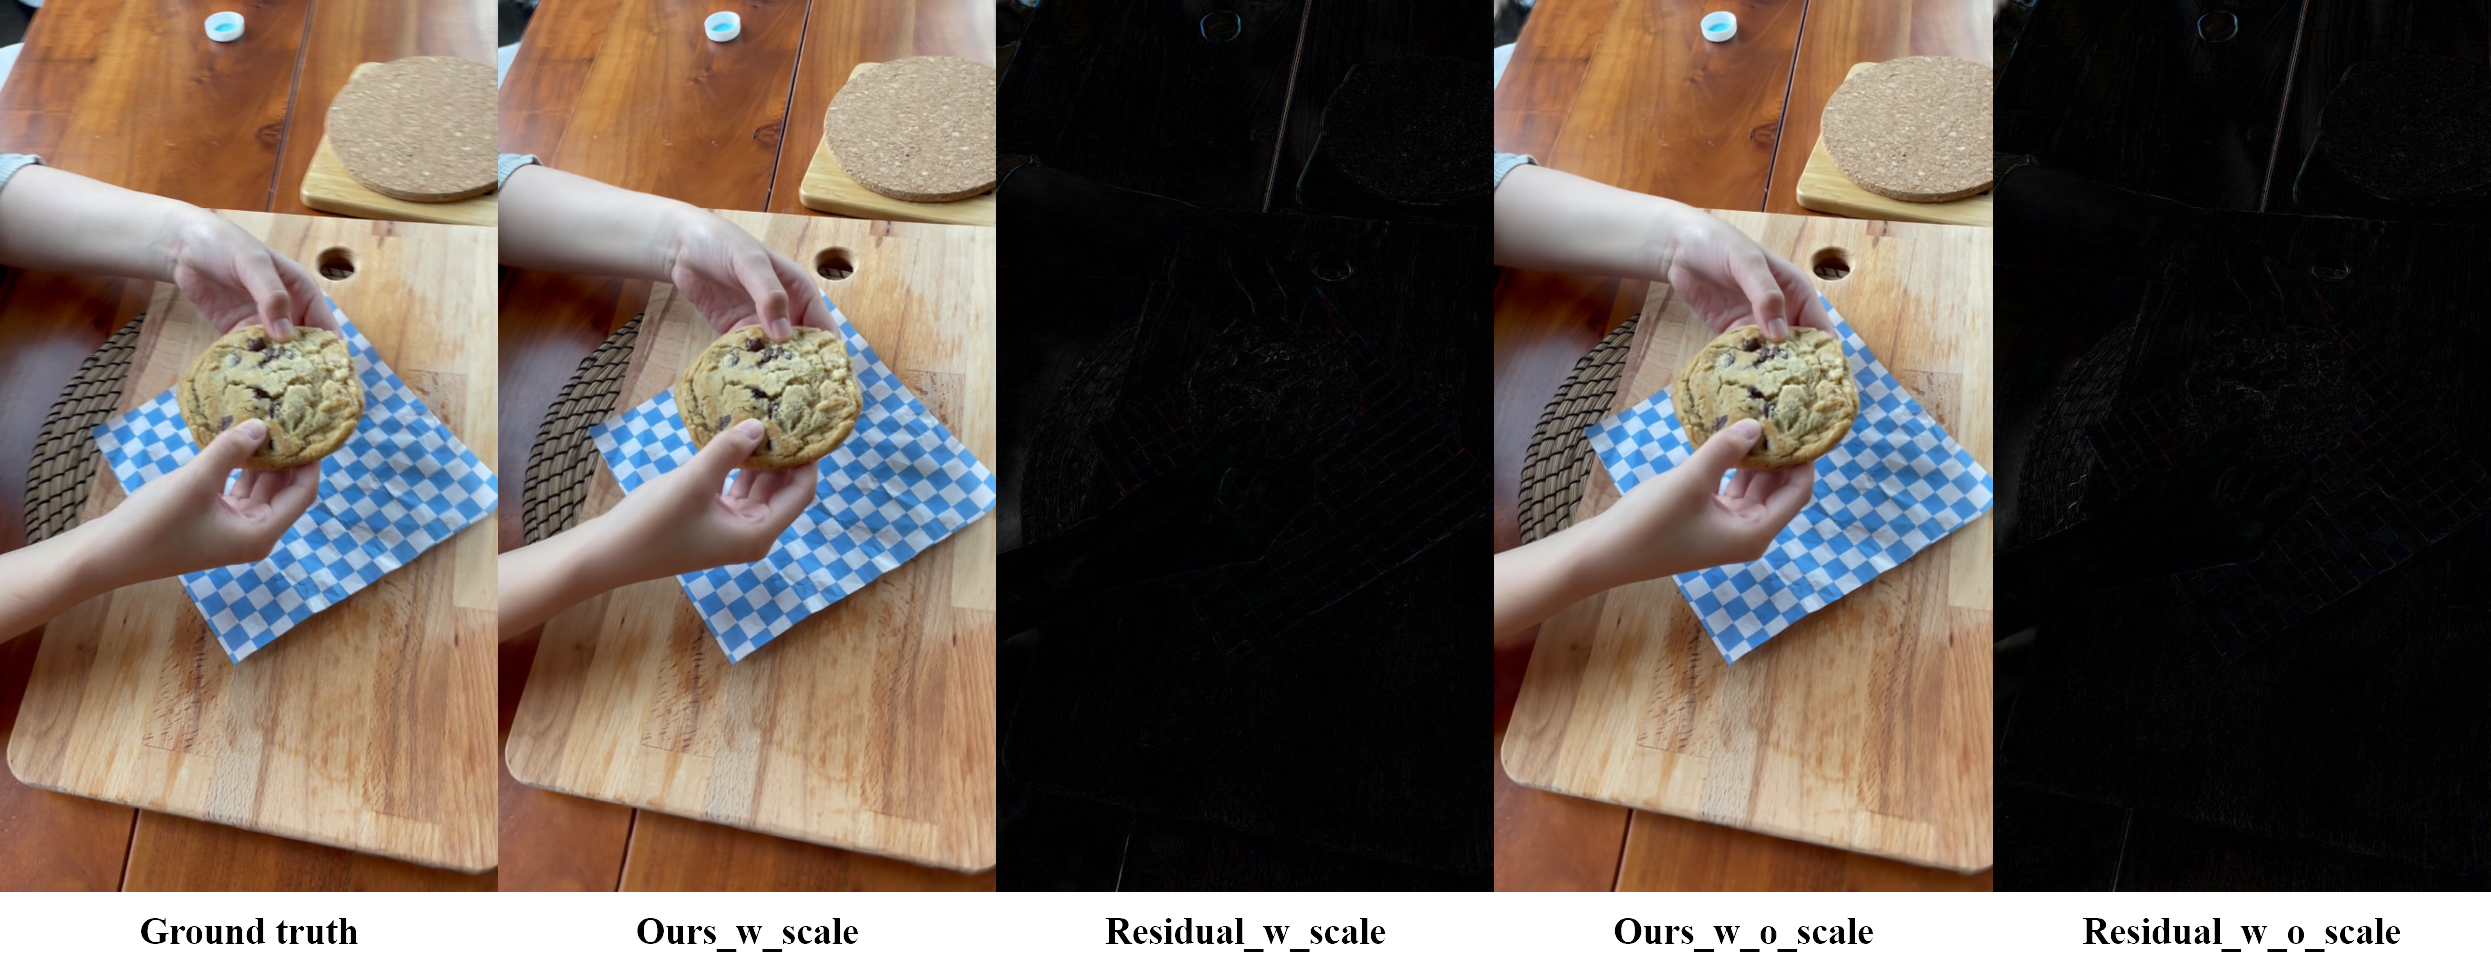
\includegraphics[width=\textwidth]{sec/fig/scale.png} 
    \vspace{-20pt}
    \caption{Comparison of residuals with and without the inclusion of scaling}
    \label{fig:scale_ablation}
\end{figure*}

\noindent{\bf Scaling}
In the Gaussian parameters (rotation, position, scaling) for shape and position, we found that optimizing the scaling parameter didn't notably improve rendering but increased training time. Consequently, in designing our deform-net, we omitted to optimize the Gaussian scaling. Results from training with and without scaling indicate a $9\%$ time difference (with scale: 102 min, without scale: 93 min).

Furthermore, the exclusion of the scaling parameter had a negligible impact on the rendering performance, with a marginal decrease in PSNR by just 0.05. Visual comparison in Figure~\ref{fig:scale_ablation} also confirms that the residual difference between the render result and ground truth is minimal, with or without the scaling parameter in the model.



% \begin{figure*}[t] 
% 	\begin{center} 
% 		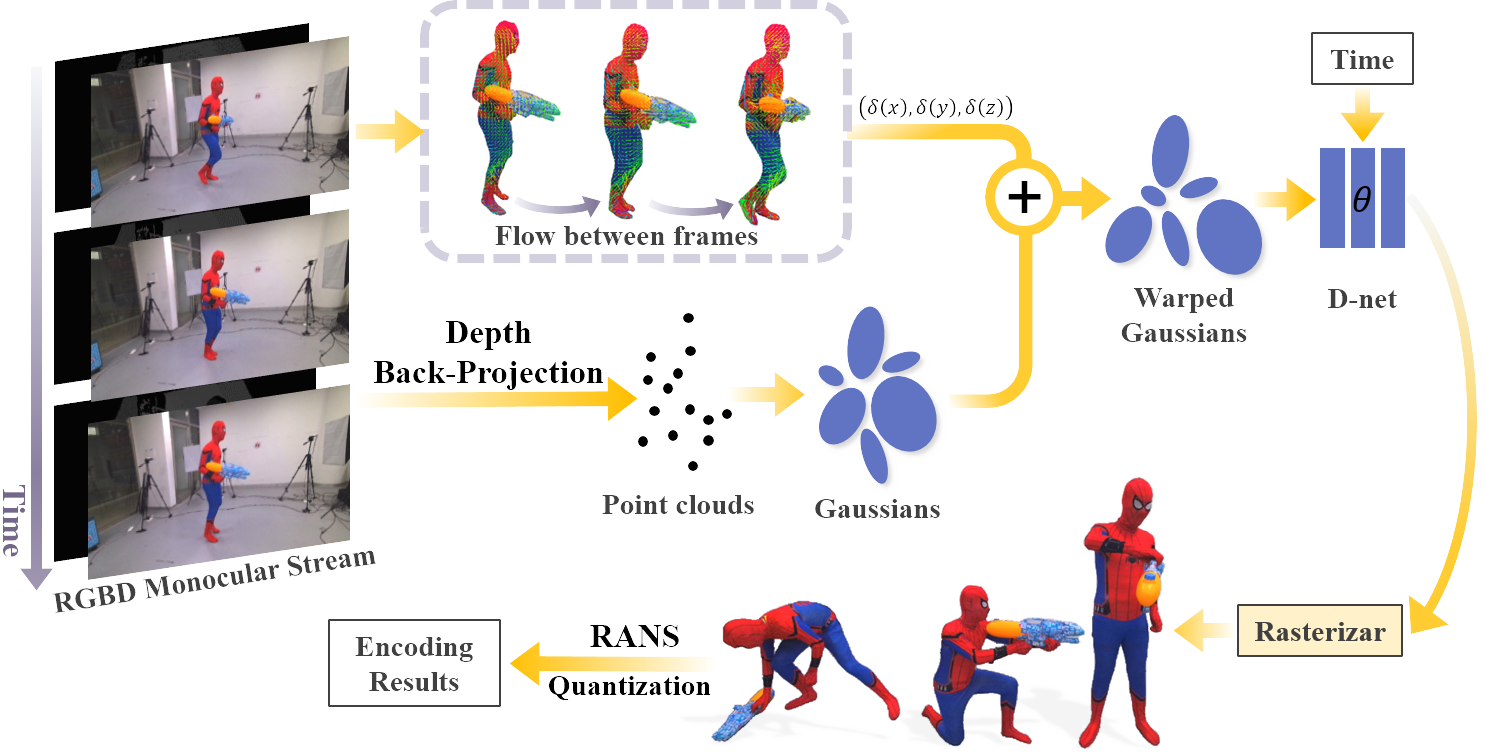
\includegraphics[width=\linewidth]{sec/fig/pipeline.png} 
% 	\end{center} 
%     \vspace{-20pt}  
% % (a)我们的setting是RGBD monocular stream (b)对depth反投影产生初始点云初始化gaussians (c)利用flow between frames对gaussians进行warp,得到的warped gaussians作为先验进入deformable net(D-net)(d)D-net额外引入time作为输入估计当前的deltax,deltay,deltaz,deltar (e)对得到的gaussians利用RANS和quantization进行压缩
%     \caption{\noindent{\bf Overview of DynTCG.} (a) Our setting involves an RGBD monocular stream. (b) DynTCG performs back-projection on the depth to generate initial point clouds and initialize Gaussians. (c) Utilizing the flow between frames, we warp the Gaussians, and the resulting warped Gaussians are used as a prior input into the deformable network (D-net). (d) The D-net additionally introduces time as an input to estimate the current $\delta(x)$, $\delta(y)$, $\delta(z)$, and $\delta(r)$. (e) After training, the Gaussians are then compressed using RANSAC and quantization.}
% 	\label{fig:fig_2_overview} 
% 	\vspace{-8pt}
% \end{figure*} 


\noindent{\bf Residual Compensation}
As illustrated in Tab.~\ref{table:residual}, we allocate 46.23MB of storage for the 4D Gaussians of each frame before compression. Applying high-bit quantization (0-bit for motion and 9-bit for appearance) without residual compensation results in a storage requirement of 7.34MB. Using low-bit quantization (11-bit for motion and 7-bit for appearance), again without residual compensation, reduces storage to 3.23MB but compromises rendering quality. In contrast, applying the same low-bit quantization but with residual compensation significantly reduces storage needs to under 2MB per frame while maintaining the same level of rendering quality.
\begin{table}[b]
    \Huge
	\begin{center}
		\centering
		\caption{Quantitative evaluation of residual compression methods.}
		\label{table:residual}
		\resizebox{0.45\textwidth}{!}{
			\begin{tabular}{l|c|c}
				\hline
				\hline
& Per-frame Storage(MB) $\downarrow$ & PSNR(dB) $\uparrow$\\
\hline
Raw Point Cloud   &  46.23 & 32.47  \\
% \hline
High-bit Quantization    &  7.34 & 32.23  \\
% \hline
Low-bit Quantization    &  3.23 & 29.56  \\
% \hline
\hline
Ours Residual Encoding    &  1.35 & 32.30  \\
\hline
\hline
			\end{tabular}
		}
		\vspace{-20pt}
	\end{center}
\end{table}

% \begin{figure*}[t] 
% 	\begin{center} 
% 		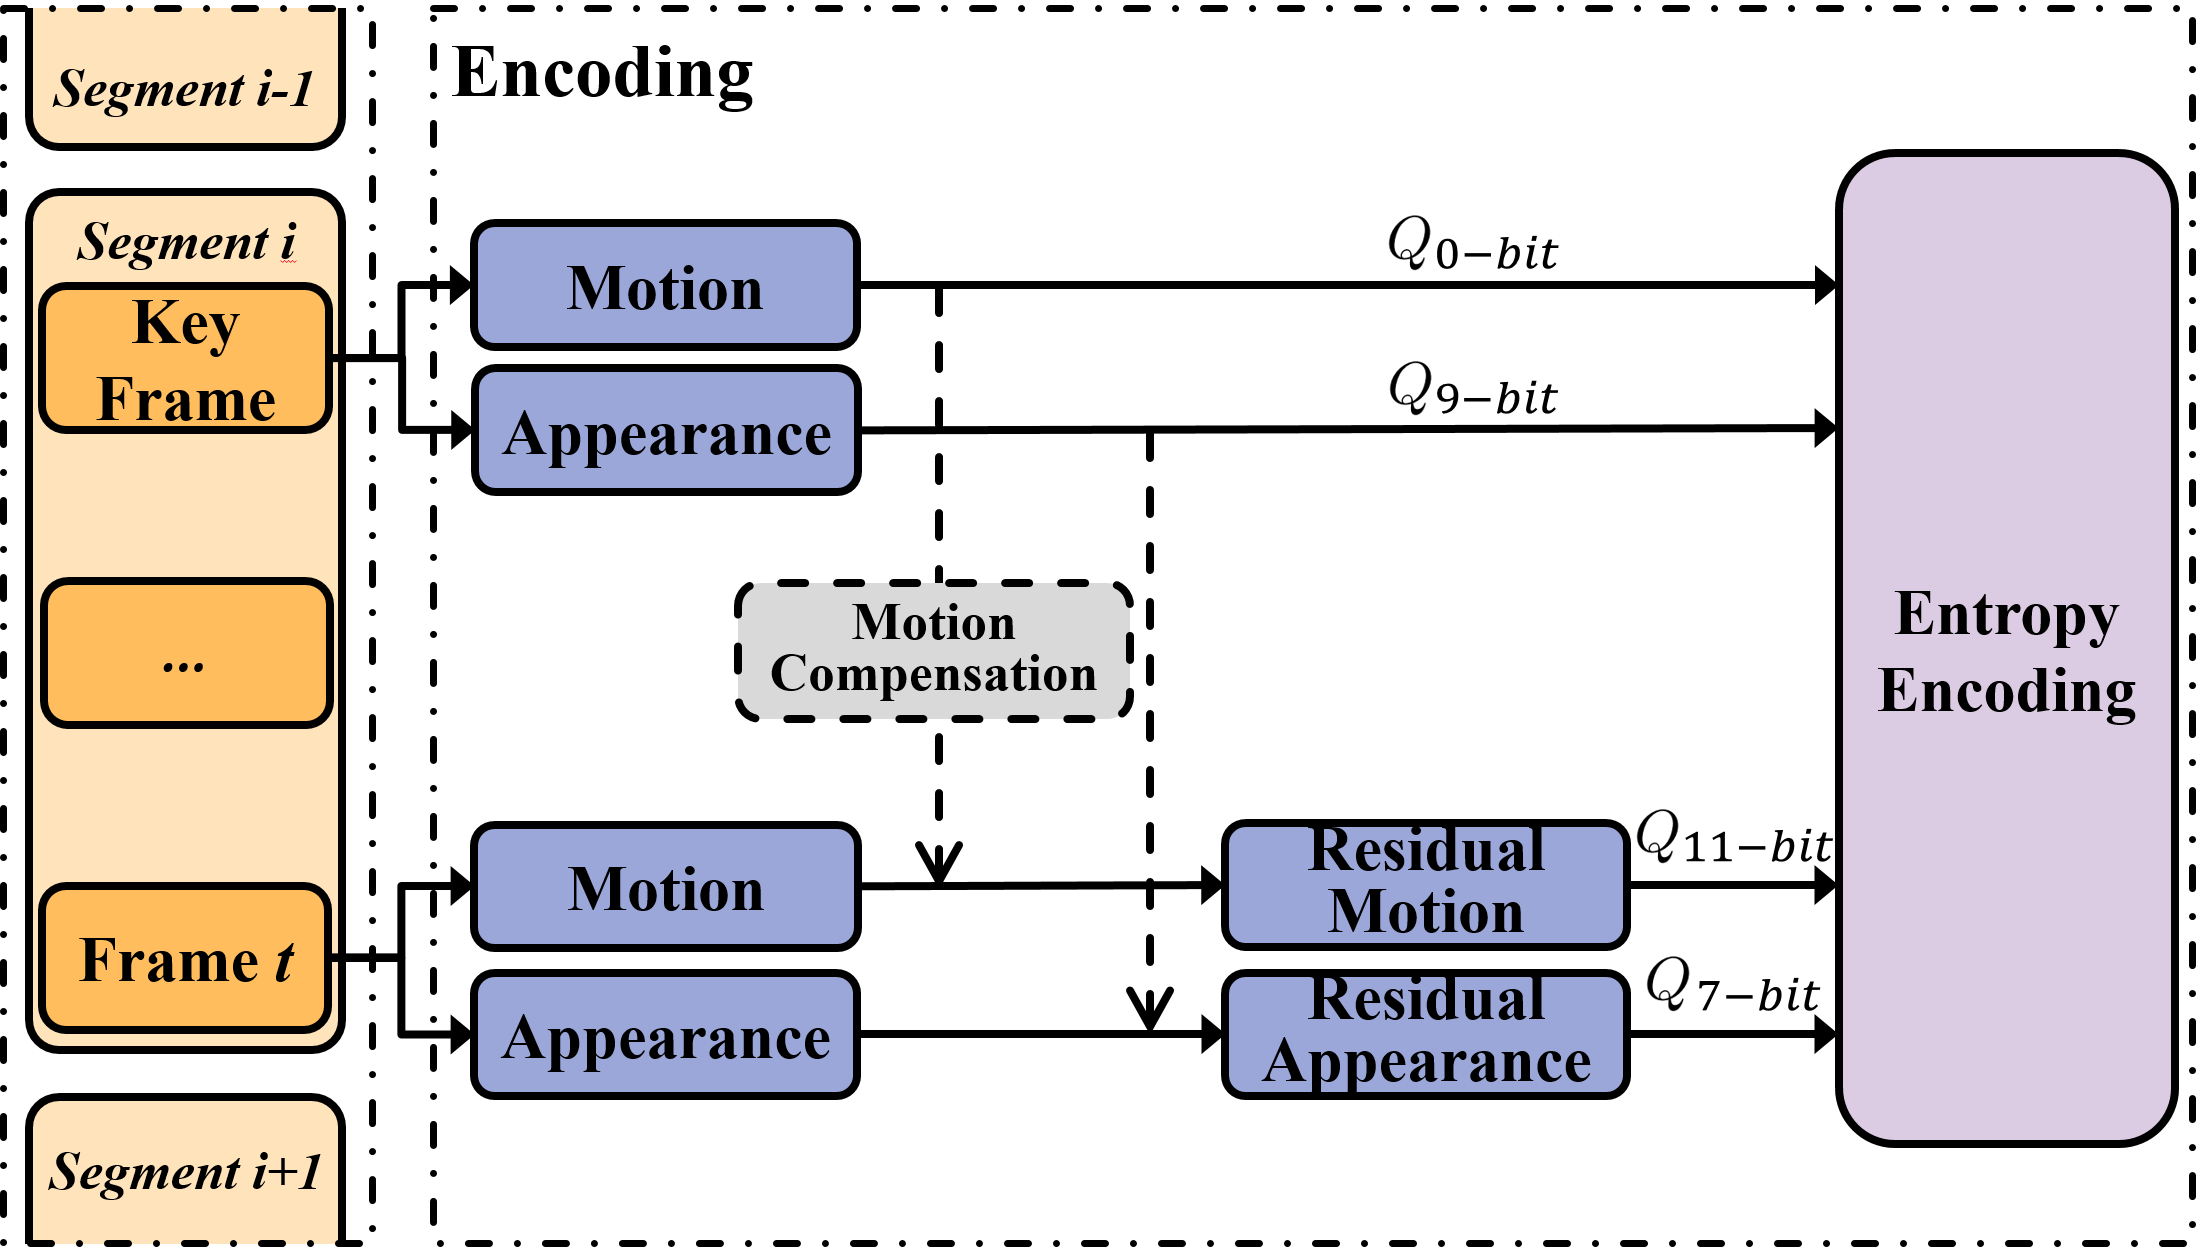
\includegraphics[width=\linewidth]{sec/fig/encoding.png} 
% 	\end{center} 
%     \vspace{-20pt}
%     \caption{Illustration of residual encoding strategy for DynTCG.}
%     \label{fig:encoding}
% \end{figure*}
% \begin{figure}[t]
% 	\centering
% 	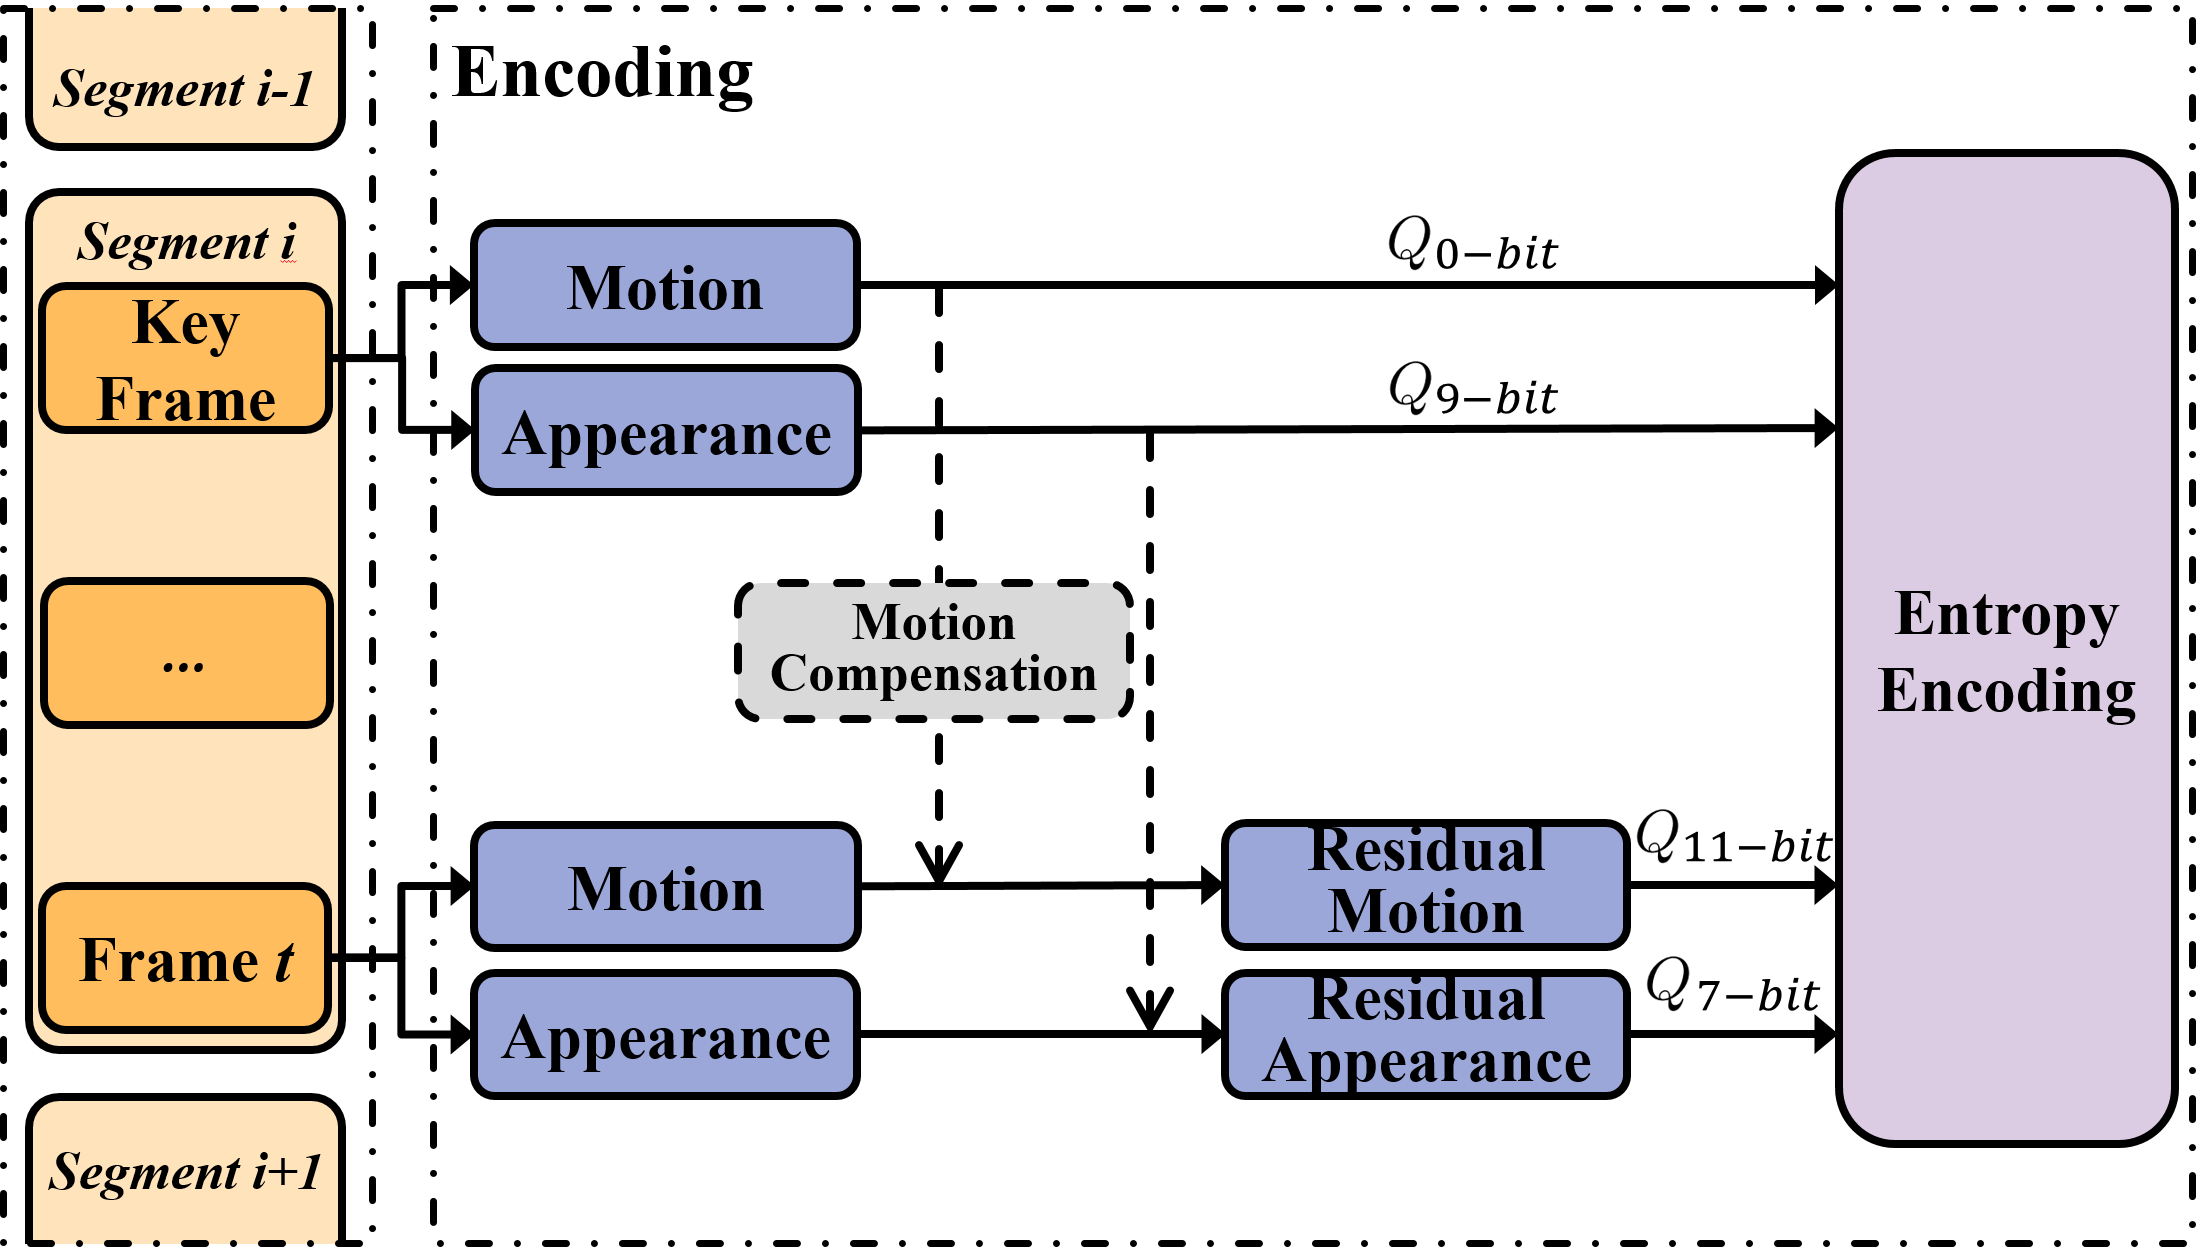
\includegraphics[width=\linewidth]{sec/fig/encoding.png}
% 	\vspace{-20pt}
% 	\caption{Illustration of residual encoding strategy for DynTCG.}
% 	\label{fig:encoding}
% \end{figure}
\subsection{Comparison}
We compare DynTCG with the methods including Instant-NVR\cite{jiang2023instantnvr}, DynamicNeRF\cite{gao2021dynamic}, and TineuVox\cite{Fang_2022} on Dynamic Scene Dataset and our captured data. As depicted in Fig~.\ref{fig:comparison}, we can observe that for areas with abundant texture and sharp edges, the reconstruction effect of Instant-NVR is mediocre, and its color prediction is also not very accurate. DynamicNeRF and Tinuvox show better overall object reconstruction, but their performance in texture detail is poor, resulting in significant blurring at the edges, to the extent that texture details become indiscernible. In contrast, our method DynTCG, based on Deformable 3D Gaussians, enhances its performance with depth map back-projection for point cloud re-projection constraints. Additionally, using Optical Flow Tracking as a prior provides a better initialization, leading to significantly improved results. Our method achieves better outcomes for complex textures, reconstructing them with greater clarity. Simultaneously, we also compare the average performance across different datasets in terms of PSNR, SSIM, and Per-frame Storage. It can be seen from the Tab.~\ref{table:Qualitativecomparison} that our metrics are superior to other algorithms in several aspects, further validating the robustness of our algorithm. The qualitative metrics prove that the rendered picture of our method surpasses other methods. What's more, the storage of our method can be reduced by about 90 percent compared with our methods, which ensures the easy preservation of each frame.
\begin{table}[t]
	\begin{center}
		\centering
		% \vspace{-25pt}
        \caption{
        Quantitative comparison of rendering results. Green and yellow cell colors indicate the best and the second-best results. %best and the second best results.
        }
		\resizebox{0.47\textwidth}{!}{
			\begin{tabular}{l|ccccc}
				\hline
				Method   &  PSNR $\uparrow$ & SSIM $\uparrow$ & Per-frame Storage(MB) $\downarrow$ \\
				\hline
                    Instant-NVR~\cite{jiang2023instantnvr} & 28.82 & 0.976 & 24.16 \\
				DynamicNeRF~\cite{gao2021dynamic}\qquad\qquad & 26.65 & 0.8452 & 21.5 \\
			    TineuVox~\cite{Fang_2022}     & 24.71 & 0.813 &  \secondBestCellColor{11.38} \\
    		\hline

                Ours(Before Compression)  & \bestCellColor{\textbf{32.47}} & \bestCellColor{\textbf{0.989}} & \textbf{43.42}\\
                Ours(After Compression) & \secondBestCellColor{\textbf{32.30}} & \secondBestCellColor{\textbf{0.983}} & \bestCellColor{\textbf{1.648}}\\
				\hline
			\end{tabular}
            }
		\label{table:Qualitativecomparison}
    
    		\vspace{-25pt}
	\end{center}
\end{table}

\section{Results}
\begin{figure}[b]
  \centering
   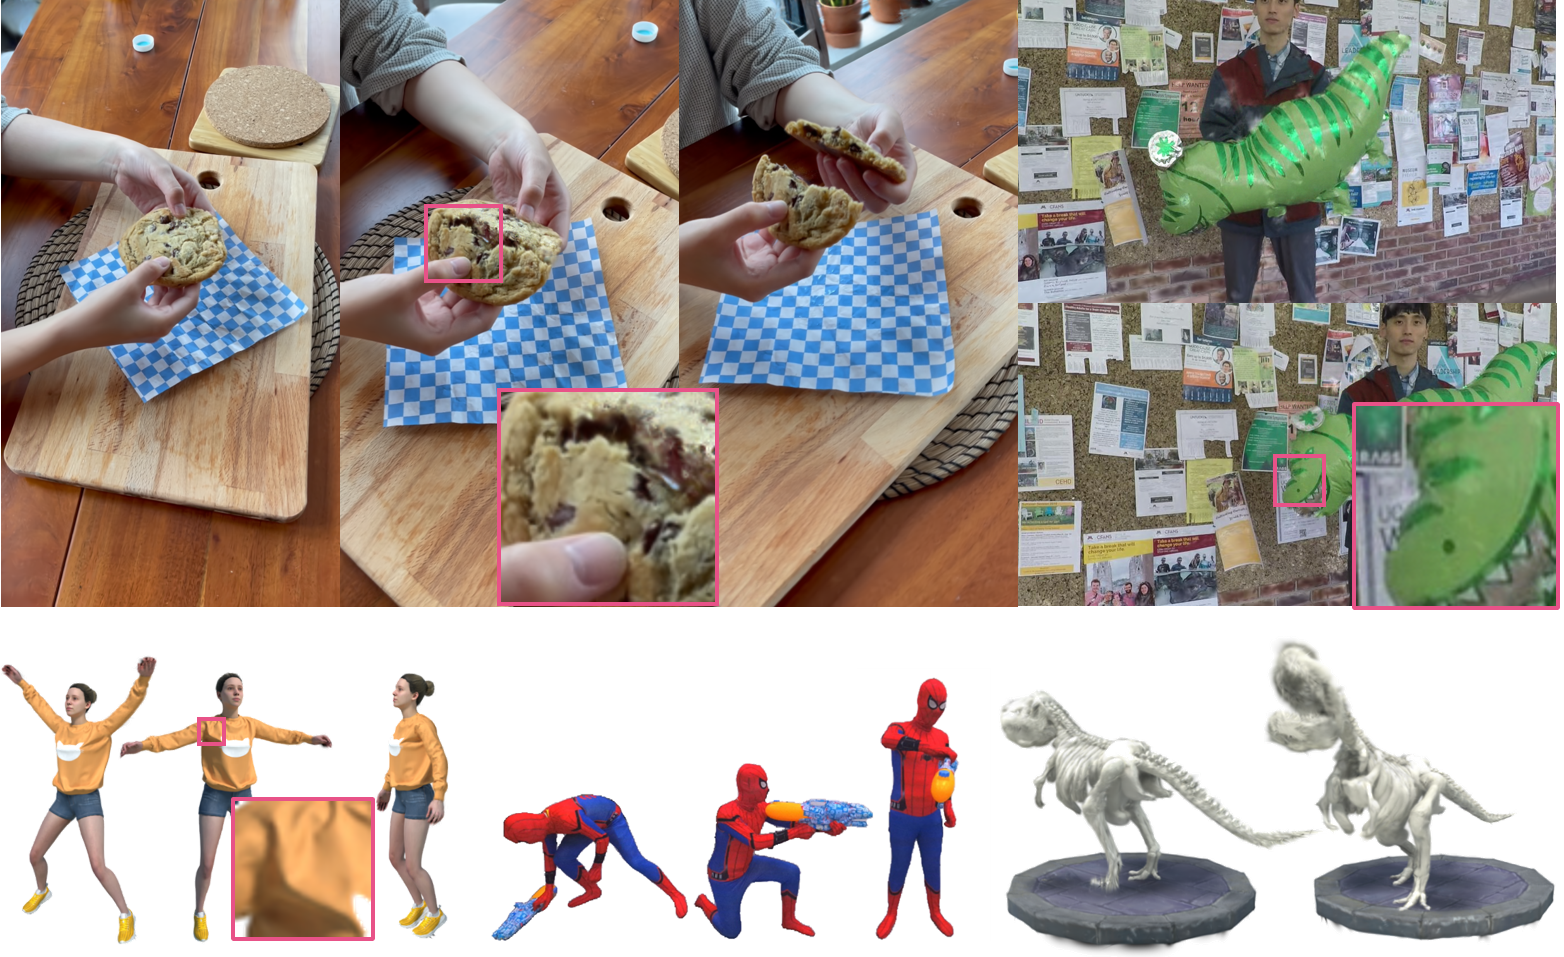
\includegraphics[width=1.0\linewidth]{sec/fig/results.png}

   \caption{The results of our method}
   \label{fig:results}
\end{figure}
The picture presented as Fig.~\ref{fig:results} demonstrates the effectiveness of our method. The top-left data originates from the HyperNeRF Dataset, with the camera setting being a pinhole camera model with tangential and radial distortion. The data in the top right is from the Dynamic Scene Dataset, captured using a moving monocular camera; it represents short-term dynamic events ($\sim$ 5 seconds) recorded with a hand-held, moving camera. The bottom-left and bottom-right data are from D-Nerf, with the camera setting being a sparse set of images of a dynamic scene, captured by a monocular camera for sparse views by moving non-rigidly. Lastly, the data in the center bottom is from the Instant-NVR dataset, captured with an RGBD Kinect camera.

\section{Limitations}
Our method still has some limitations. The DynTCG takes RGBD images as input, which requires an RGBD camera to capture. Though we could use monodepth to estimate depth from RGB images, the error in depth estimation can lead to a bad effect on the back-projection module. Besides, our optical flow tracking will fail to deal with a non-continuous image input, limiting the data set to continuous captures. 

\section{Conclusions}
We have presented a deformable Gaussian representation that takes monocular RGBD input and synthesizes a dynamic novel view. By utilizing optical flow tracking from 2D images into deformable dynamic Gaussian-splatting, our approach achieves high-fidelity rendering results, outperforming previous methods in terms of quality, training speed, and storage. Our optical flow and Gaussian point cloud wrap method provides a favorable prior, achieving a great acceleration on the deformable network training speed. We also present a residual encoding method to address the long sequence storage problem, by applying quantization and RANS Encoding on the residual point cloud, we achieve a compression rate of 25, making long dynamic sequences loading and training. Our experimental results show that our method outperforms other monocular methods under the same settings. We believe our method achieves a critical step in monocular dynamic novel view synthesis. 


\section{Acknowledgement and Contribution}
% \begin{enumerate}
%     \item Baseline (the development of D-net) (Hong Yu, Shen Zhehao)
%     \item Apply flow tracking as a powerful prior to D-net (Shen Zhehao)
%     \item Modify the D-net (remove the scale and improve the training speed) (Zhou Shouchen)
%     \item Use the Quantization and RANS Encoding to compress Gaussians (Wang Penghao)
%     \item Residual compression design (Wang Penghao, Zhang Zhirui)
%     \item Dynamic viewer development (Zhang Zhirui)
%     \item Comparison experiment (Shen Zhehao, Hong Yu, Zhang Zhirui, Wang Penghao, Zhou Shouchen)
%     \item Ablation experiment (Shen Zhehao, Wang Penghao, Zhou Shouchen)
%     \item Poster design (Hong Yu)
% \end{enumerate}
% % 此外,我们在Yuheng Jiang的帮助下在对比实验中跑通了instant-nvr的结果,感谢他的帮助
We extend our gratitude to Yuheng Jiang for his assistance with the implementation of the Instant-NVR results in comparison experiments.

The contributions to this work are as follows: Yu Hong and Zhehao Shen developed the initial baseline through the design of the deform net. Zhehao Shen further enhanced this by integrating flow tracking as an effective prior. Shouchen Zhou contributed significant improvements to the deform net by removing redundant scale parameters and optimizing training speed. Penghao Wang introduced a novel approach to Gaussian compression using Quantization and RANS Encoding, as well as collaborating with Zhirui Zhang on the residual compression design. Zhirui Zhang also spearheaded the development of the dynamic viewer. Comparative and ablation experiments were conducted by Zhehao Shen, Yu Hong, Zhirui Zhang, Penghao Wang, and Shouchen Zhou, with Yu Hong taking the lead on poster design.


{
    \small
    \bibliographystyle{ieeenat_fullname}
    \bibliography{main}
}

% WARNING: do not forget to delete the supplementary pages from your submission 
% \clearpage
\setcounter{page}{1}
\maketitlesupplementary


\section{Rationale}
\label{sec:rationale}
% 
Having the supplementary compiled together with the main paper means that:
% 
\begin{itemize}
\item The supplementary can back-reference sections of the main paper, for example, we can refer to \cref{sec:intro};
\item The main paper can forward reference sub-sections within the supplementary explicitly (e.g. referring to a particular experiment); 
\item When submitted to arXiv, the supplementary will already included at the end of the paper.
\end{itemize}
% 
To split the supplementary pages from the main paper, you can use \href{https://support.apple.com/en-ca/guide/preview/prvw11793/mac#:~:text=Delete%20a%20page%20from%20a,or%20choose%20Edit%20%3E%20Delete).}{Preview (on macOS)}, \href{https://www.adobe.com/acrobat/how-to/delete-pages-from-pdf.html#:~:text=Choose%20%E2%80%9CTools%E2%80%9D%20%3E%20%E2%80%9COrganize,or%20pages%20from%20the%20file.}{Adobe Acrobat} (on all OSs), as well as \href{https://superuser.com/questions/517986/is-it-possible-to-delete-some-pages-of-a-pdf-document}{command line tools}.

\end{document}
